% document formatting
\documentclass[10pt]{article}
\usepackage[utf8]{inputenc}
\usepackage[left=1in,right=1in,top=1in,bottom=1in]{geometry}
\usepackage[T1]{fontenc}
\usepackage{xcolor}

% math symbols, etc.
\usepackage{amsmath, amsfonts, amssymb, amsthm}

% lists
\usepackage{enumerate}
\usepackage{enumitem}

% images
\usepackage{graphicx} % for images
\usepackage{tikz}
\usetikzlibrary{arrows.meta}

% code blocks
% \usepackage{minted, listings} 

% verbatim greek
\usepackage{alphabeta}

% custom commands
\newcommand{\rank}{\text{Rank}}
\newcommand{\select}{\text{Select}}

\graphicspath{{./assets/images/Week 10}}

\title{02-614 Week 10 \\ \large{String Algorithms}}
 
\author{Aidan Jan}

\date{\today}

\begin{document}
\maketitle

\section*{Applications of Wavelet Trees}

\subsection*{Application 1: Document Retrieval}
Given documents $D_1, \dots, D_m$, and given a word $w$, return which documents contain $w$.
\begin{itemize}
	\item A document is a list of words.  i.e., strings over $\Sigma = \{\text{words}\}$.  that is, an entire English word is a symbol in our alphabet.
\end{itemize}
For this problem, we can first create a string $S$, which is all the documents concatenated with unique terminator characters between them.  i.e.,
\[S := D_1\$_1 D_2\$_2 \dots D_m \$_m\]
Pseudocode:
\begin{verbatim}
i = 1
while (i <= |S|):
    p_i = Select_w(i)       // Find the i-th occurance of our word
    d_i = Rank_$(p_i) + 1   
    output d_i
    p' = Select_$(d_i)      // Get end of document with i-th word
    i = Rank_w(p') + 1      // Skip past the word occurrence in current document
\end{verbatim}
\begin{itemize}
	\item Recall that each word is a character in $S$.  Therefore, $|S|$ refers to the total number of words across all documents.
	\item Wavelet trees are used to implement Select and Rank.  The $|\Sigma|$ would be the size of the English dictionary.
	\item Runs in $O(\log |\Sigma|)$.  The number of loops is equal to the number of documents output.
\end{itemize}

\subsection*{Application 2: Storing graphs}
Wavelet trees can also be used to store graphs.  Consider the following graph:
\begin{center}
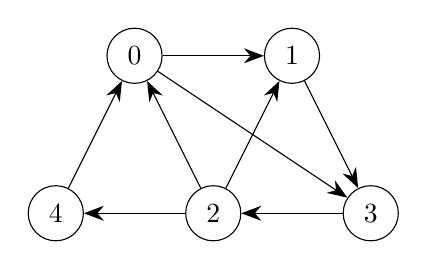
\begin{tikzpicture}
    \node[draw, circle, minimum size=0.7cm] at (0, 0) (0) {$0$};
    \node[draw, circle, minimum size=0.7cm] at (2, 0) (1) {$1$};
    \node[draw, circle, minimum size=0.7cm] at (1, -2) (2) {$2$};
    \node[draw, circle, minimum size=0.7cm] at (3, -2) (3) {$3$};
    \node[draw, circle, minimum size=0.7cm] at (-1, -2) (4) {$4$};

    \draw[-{Stealth[scale=1.5]}] (0) -- (1);
    \draw[-{Stealth[scale=1.5]}] (0) -- (3);
    \draw[-{Stealth[scale=1.5]}] (1) -- (3);
    \draw[-{Stealth[scale=1.5]}] (2) -- (4);
    \draw[-{Stealth[scale=1.5]}] (2) -- (0);
    \draw[-{Stealth[scale=1.5]}] (2) -- (1);
    \draw[-{Stealth[scale=1.5]}] (3) -- (2);
    \draw[-{Stealth[scale=1.5]}] (4) -- (0);
\end{tikzpicture}
\end{center}
\begin{verbatim}
Node | Out-neighbors
0    | 1, 3
1    | 3
2    | 0, 1, 4
3    | 2
4    | 0
\end{verbatim}
To store a graph, we basically need two functions:
\begin{itemize}
	\item $\text{succ}(u, i)$ = $i$-th node pointed to by $u$
	\item $\text{pred}(u, i)$ = $i$-th predecessor (parent) of $u$
\end{itemize}
We can first make a data structure:
\begin{itemize}
	\item $A = [1, 3, 4, 0, 1, 2, 0]$
	\item $B = [1, 0, 1, 1, 0, 1, 1]$
\end{itemize}
$A$ represents outneighbors of nodes in clockwise order (This ordering does not really matter.), with node 0 first, then node 1, etc., all concatenated into an array.  $B$ stores where a node's adjacency list begins.
\begin{itemize}
	\item $A$ is stored in a wavelet tree while $B$ is an RRR vector.
	\item The number of $1$'s in $B$ always represents the number of nodes in the graph.  The index of a $1$ in $B$ represents the index that the $i$-th adjacency list in $A$ starts.
\end{itemize}
Now, we can implement the functions:
\begin{itemize}
	\item $\text{succ}(u, i) :=$
	\begin{verbatim}
p = Select_i (B, u + 1)     // O(1)
return A[p + i]             // O(log |E|)
    \end{verbatim}
    \item $\text{pred}(u, j) :=$
    \begin{verbatim}
p = Select_u(A, j)          // O(log |E|)
return rank_1(B, p)         // O(1)
    \end{verbatim}
\end{itemize}
Note that $|E|$ is also the length of the lists.\\\\
What happens if we have a node with zero out-degree?
\begin{itemize}
	\item There are two options: we can either include a special character (e.g., $-1$) to denote that a node has no out-neighbors
	\item Or, instead of using an RRR-vector as the $B$-array, we can just have one array with \$ between each adjacency list.  The implementation of the algorithm would be similar to Application 1 in this case.
\end{itemize}

\section*{FM-Index}
First, recall the BWT search algorithm.  Given $S$ and $T$, we want to find where $S$ appears in $T$.  
\begin{itemize}
	\item To do this, we first do BWT on $T$.  Then, we calculate the left column.  We now have LF-mapping.
	\item Now, search $S$ backwards, looking for the the character on the right side.  Use the LF-mapping to search the left side.  Repeat until entire string is found.
	\item The only thing is that we somehow need to know where the $i$-time the character appears on the right.
	\begin{itemize}
	    \item \textbf{Option 1:} This happens to be the rank$_\text{c}$() function, which wavelet trees are amazing for.
	    \item \textbf{Option 2:} Use the FM-Index.
	    \[\tilde{T} = \text{Huffman}(RLE(MTF(BWT(T))))\]
        \begin{itemize}
            \item BWT = Burrows Wheeler Transform
            \item MTF = Move to front compression
            \item RLE = Run length encoding
            \item Huffman = Huffman encoding
        \end{itemize}
    \end{itemize}
\end{itemize}
For Option 2, we just have to make this super-compressed string searchable.  First, consider the BWT of $T$. 
\begin{itemize}
	\item We break the $BWT(T)$ into blocks of $u$ characters.  With this representation, if we also break the compressed string $\tilde{T}$ into blocks such that each block in $\tilde{T}$ corresponds to a block in $BWT(T)$, the blocks might not be the same size, but they will be in the same order.
	\item Now, if $\tilde{T}$ is represented in terms of blocks $BZ_1, BZ_2, \dots, BZ_b$, where $b$ is the number of blocks in total, we can now represent this as \textit{super-blocks}.  A super-block is a block containing $u$ blocks.
	\item Now we can start storing stuff.  Make an array of size $|\Sigma|$ (one array index per alphabet character) \textit{per superblock}, and it stores the number of occurrences of the given character up to and including the superblock $b$.
	\item Make another set of arrays of size $|\Sigma|$, one for each block in $BWT(T)$, and have each index store the number of characters up to the end of the block in $BWT(T)$, since the end of the last superblock.
	\item To search the rank of a character, first check its occurrence in its block, then check the number of occurrences in the previous superblocks.
\end{itemize}
How big is this data structure?
\begin{itemize}
	\item We have a total of $n / u$ block (excluding superblock) arrays.  This takes advantage that there are $u$ characters per block in BWT of $T$.
	\item Recall that each block array stores counts of letters.  Therefore, every count must be smaller than $u^2$.  
	\item Therefore, we need a total of $\frac{n}{y} \left(\log u^2\right) |\Sigma|$ bits to store the block array.  If we assume $u = O(\log n)$, then the space taken up by block arrays is $O(\frac{n}{\log n} \log \log n)$.  This approaches zero when $n$ is large!
	\item Now for superblocks, we have a total of $(\frac{n}{u}) / u$ total superblocks.  Size of each super block array is $|\Sigma| \log n$.  Calculating the bits required for the superblock, we get $n / \log n$.  This is even smaller than the block arrays.
\end{itemize}





\end{document}
